\documentclass{article}
\usepackage[utf8]{inputenx}
\usepackage{graphicx}
\newcommand{\equ}{EQU}
\title{\equ\\
  Diseño y Especificación}
\begin{document}
\maketitle

\section{Introducción}
\label{sec:intro}
El objetivo general de \equ\ es realizar demostraciones, automáticamente
verificadas, de fórmulas escritas en una lógica ecuacional. Las fórmulas
pueden incluir términos de diferentes \emph{teorias} (aritmética, listas,
lógica proposicional, lógica de primer orden, etc), cada una de las cuales
incluyen un conjunto de símbolos predefinidos (operadores y constantes). En
términos mas generales, \equ\ permite construir demostraciones de que cierta
expresión (de cualquier tipo, aunque preferiblemente fórmulas) se puede
reescribir como otra expresión (preferiblemente \emph{canónica}).

\section{Caso de uso típico}

El siguiente caso de uso muestra las características principales del sistema
desde la perspectiva del usuario. Se destacan las principales estructuras de
datos (en \textbf{negrita}), los principales algoritmos (en \emph{cursiva}), y
las características fundamentales de la interfaz de usuario. Las estructuras
de datos y algoritmos muy posiblemente requieran de otras estructuras de datos
auxiliares.

\begin{figure}[t]
  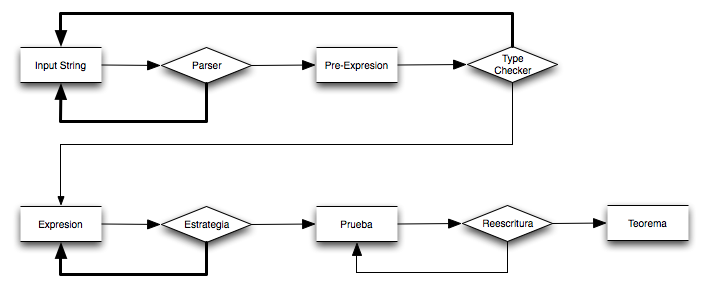
\includegraphics[scale=0.5]{flow_equ.png}  
  \label{flow_equ}
  \caption{Flujo de información}
\end{figure}


\label{sec:usecase}
\begin{enumerate}
\item El usuario ingresa un \textbf{string}, que pretende ser la representación
  textual de una expresión. 
  
\item El sistema intenta \emph{parsear} dicha entrada, reconociendo los símbolos 
  predefinidos en las teorías soportadas, nombres de variables, y nombres
  de operadores definidos \emph{ad-hoc} por el usuario, respetando
  el parentizado dado en caso de estar presente. El parser debe resolver
  cuestiones de precedencia y asociatividad. 
  
  Si el parseo falla de deben dar los mensajes de error informativos. El usuario
  tiene la posibilidad de corregir el \textbf{string} de entrada.
  
  Si el parseo es exitoso se genera una \textbf{pre-expresión}.
  
  El sistema debería soportar un modo de entrada interactivo, que construya
  \textbf{pre-expresiones} con ``huecos'' para los parámetros de cada operador, 
  de forma que el parseo sea siempre efectivo, una vez completados todos los
  ``huecos''.
  
\item Una \textbf{pre-expresión} (completa) mantiene una estructura arbórea de la 
  expresión pretendida. Una \textbf{pre-expresión} se puede generar cuando
  cada símbolo está aplicado a un número correcto de \textbf{pre-términos},
  aunque estos \textbf{pre-términos} no sean del tipo adecuado.
  
\item El sistema intenta \emph{chequear tipos} sobre la \textbf{pre-expresión}.
  El chequeo de tipos consiste básicamente en inferir tipos para las variables
  y verificar la correcta aplicación de cada operador.
  
  Si el chequeo falla el usuario tiene la posibilidad de corregir la entrada.
    
  Si el chequeo es exitoso entonces se construye una \textbf{expresión}.
  
  El chequeo se debería poder realizar partiendo de ciertas restricciones
  impuestas por el usuario (incluso el árbol de tipos completo). 
  En caso de fallo, se debería guiar al usuario a encontrar el error. O bien
  se fuerza a que el usuario explicite los tipos inconsistentes para las
  variables no-unificables, o bien se permite que redefina el tipo del operador
  (temporalmente). De esta forma se pretende que se hagan mas evidentes
  los errores y se pueda aprender de ellos.
    
\item Dada una expresión se elige una \emph{estrategia} para su reducción
  a forma normal. Normalmente será una estrategia de prueba para reducir una
  formula. La estrategias posibles dependen del tipo de la expresión. Por 
  ejemplo, una expresión aritmética sólo aceptara una estrategia de
  reducción directa, aplicando pasos de ``unfolding'' de los operadores
  involucrados. Una expresion del tipo fórmula podría aceptar diversas 
  estrategias: análisis por casos, inducción (si involucra expresiones 
  aritméticas o de listas), absurdo, etc.
  
  La estrategia puede no ser adecuada para el tipo de expresión, y en tal caso
  se permite volver a elegir.
  
  Si la estrategia es adecuada, se genera una \textbf{prueba}, que debe ser 
  completada.
  
\item Una \textbf{prueba} es un conjunto de una o mas expresiones que
  que deben ser reducidas, y para cada una de ellas, una secuencia de pasos de 
  re-escritura que demuestran la reducción. Cada paso de reescritura esta
  justificado por un axioma (propio de la teoria), definicion de operador
  (predeterminado en la teoria o definido por el usuario) o un \textbf{teorema}
  (dado por la relación entre una expresión y su forma reducida, una vez
  que ha sido demostrada).
  
\item Una vez que que cada expresión a sido reducida a su forma canónica, 
  la prueba de reducción se considera terminada.
\end{enumerate}

\end{document}
